\documentclass[11pt]{article}
\usepackage[margin=1in]{geometry}
\usepackage[T1]{fontenc}
\usepackage{lmodern}
\usepackage{microtype}
\usepackage{booktabs}
\usepackage{tabularx}
\usepackage{xcolor}
\usepackage{enumitem}
\usepackage{pgfplots}
\pgfplotsset{compat=1.18}
\usepackage[hidelinks]{hyperref}
\usepackage{natbib}

\definecolor{series}{HTML}{2A78D6}
\definecolor{inkmuted}{HTML}{52514E}
\definecolor{gridc}{HTML}{E4E3DF}

\pgfplotsset{
  attbar/.style={
    ybar, bar width=14pt, ymin=0,
    axis x line*=bottom, axis y line*=left,
    ymajorgrids, grid style={gridc},
    tick label style={font=\small, text=inkmuted},
    label style={font=\small},
    every axis plot/.append style={fill=series, draw=none},
    nodes near coords, nodes near coords style={font=\scriptsize, text=inkmuted},
    enlarge x limits=0.08,
    width=0.95\linewidth, height=5.2cm,
  }
}

\title{\textbf{Local-First Teams of Coding Agents:}\\
A Field Study of 344 Merged Tasks in Nine Days\\
with a Supervised PM / Tech-Lead / Coder Architecture}
\author{Ali Mohammad\\Independent researcher\\\texttt{<email>}}
\date{October 2026}

\begin{document}
\maketitle

\begin{abstract}
Coding agents now resolve isolated issues well, but a product is not a set of
isolated issues: it needs someone to decide what is wrong, someone to write the
fix, someone to check it, and a way for all of them to share one repository
without colliding. We present \textbf{ATT} (Agent Team Template), an open,
\emph{local-first} operating model for a team of Claude Code agents running on a
single developer machine: a product manager (PM) agent that runs the product
and files provable backlog rows, several coding agents that claim rows and open
pull requests, several tech-lead agents that review and merge them behind a
guarded merge, and an agent manager that the human owner talks to. Coordination
uses only artefacts a developer already has (a Markdown backlog, git commits,
GitHub labels, file locks), and every agent runs as a chain of short, fresh
sessions under a supervisor that survives usage limits. We report a field study
of one local deployment on a private, actively developed project. Over
nine days, about 430 backlog rows were filed and 344 claimed rows were merged,
at a median of \textbf{1.3 hours} from claim to merge (IQR 0.6--3.2\,h; 91\%
within 8\,h), with two reverts on the integration branch. Once the supervisor
was introduced, median claim-to-merge latency fell from 10.7\,h ($n{=}30$) to
1.2\,h ($n{=}314$). This comparison is observational and confounded. We describe
the design, the measurement method, the 83 failure-driven ``lessons'' the agents
accumulated, and the threats to validity. We also propose a controlled
benchmark protocol for future work. The template is released as open source.
\end{abstract}

\section{Introduction}

Benchmarks such as SWE-bench~\citep{jimenez2024swebench} made autonomous issue
resolution measurable, and agent scaffolds such as
SWE-agent~\citep{yang2024sweagent}, OpenHands~\citep{wang2024openhands} and
Agentless~\citep{xia2024agentless} have pushed resolution rates up quickly.
These settings share an assumption: a task arrives fully specified, one agent
works on it alone, and success is a hidden test. Day-to-day product work
differs on each count. Someone must \emph{find} what is wrong with the product
and write it down so that it can be checked. Several fixes are in flight at
once, against one moving branch. Someone other than the author must check each
fix before it lands. And everything runs on the developer's own machine and CI,
whose memory and time are finite.

Multi-agent frameworks such as MetaGPT~\citep{hong2023metagpt},
ChatDev~\citep{qian2023chatdev} and AutoGen~\citep{wu2023autogen} model
software roles inside one conversation or one process. ATT takes a different
position: \textbf{the roles are separate, long-lived processes, and they
coordinate only through the repository}. A backlog row, a claim commit, a PR
label and a lock file are the whole protocol. This has three consequences that
we found decisive in practice:
\begin{enumerate}[leftmargin=*,itemsep=2pt]
  \item \emph{Context stays small.} No agent holds the team's state in its
        context. Each session does one unit of work and exits, which avoids the
        known degradation of long contexts~\citep{liu2023lost}.
  \item \emph{It is local-first.} The team runs on one owner machine, under
        \texttt{systemd} user units, against the owner's own CI runners. No
        hosted orchestration service is involved, and the owner can inspect or
        stop any agent with ordinary tools.
  \item \emph{Failures become rules.} Each role keeps a numbered
        \texttt{lessons.md}. A failure that cost a run becomes a written rule
        that later sessions read, which is a persistent, human-auditable
        analogue of verbal self-reflection~\citep{shinn2023reflexion}.
\end{enumerate}

\paragraph{Contributions.}
(i) A role and protocol design for a team of coding agents sharing one
repository and one machine (\S\ref{sec:design}). (ii) An open-source
implementation for Claude Code~\citep{claudecode}: skills, shared docs and a
supervisor~\citep{att}. (iii) A field study of one deployment, measured from
git history alone (\S\ref{sec:method}--\ref{sec:results}). (iv) A catalogue of
the failure modes that the agents' lessons record (\S\ref{sec:lessons}), and a
benchmark protocol for a controlled evaluation (\S\ref{sec:future}).

\section{Design}\label{sec:design}

\subsection{Roles}
\begin{center}
\small
\begin{tabularx}{\linewidth}{@{}lXX@{}}
\toprule
Role & Does & Never \\
\midrule
PM & runs the product end to end on real inputs; judges the output; files numbered rows with a level and a \emph{done when}; in \emph{goal mode}, researches a feature into a brief and rows & reviews or merges PRs \\
Coding agent & claims a \texttt{ready} row at its level; writes a failing test; fixes the row on \texttt{agent/NN-slug}; opens a PR in a fixed template; at most two rows per session & merges; writes rows; runs heavy work locally \\
Tech lead & reviews PRs against the row's \emph{done when}, using the diff, the PR's tests and CI; starts a guarded merge; builds merge trains; keeps CI green & runs the product; numbers rows \\
Agent manager & the owner's own session: starts, stops and reports on the team; relays decisions; fixes the machinery & the agents' own work \\
\bottomrule
\end{tabularx}
\end{center}

\subsection{The backlog protocol}
A single Markdown file, \texttt{docs/BACKLOG.md}, is the only list of open
work. Each part of it has exactly one writer. The PM writes rows, their
\emph{level} (L1: one or two files with the fix named; L2: logic across a few
files following a pattern; L3: a new instrument or work that must be proven on
real fixtures), and their \emph{done when}, which must name a real artefact
and a number. A coding agent's only edit is the \textbf{claim}: a commit
changing one state cell from \texttt{ready} to \texttt{claimed agent/NN-slug},
pushed directly to the integration branch. Two agents claiming the same row is
a git push race that one of them loses, so mutual exclusion comes from git
itself. Leads own a row's state while its PR is open, and the \emph{Merged}
table. The \emph{Inbox} is a one-way channel from the leads to the PM.

\subsection{Sessions and the supervisor}
Every agent is a chain of short sessions. A session reads a per-agent
\emph{handoff} file, does one unit of work (a coder: finish open PRs, then at
most two claims; a lead: review until nothing is left to take; the PM: one
live run or one backlog pass), rewrites the handoff, and writes one status
line, \texttt{DONE}, \texttt{IDLE} or \texttt{BLOCKED}. A Bash supervisor
(about 450 lines) runs each agent under a \texttt{systemd} user unit. It
creates and signs the agent's git worktree, gates new sessions on free memory
and load, waits out account usage limits, resumes the \emph{same} session after
the reset, and stops the agent and notifies the owner on \texttt{BLOCKED}. The
PM and the leads run as interactive background sessions with Remote Control
enabled, so the owner can join any of them from a phone; the supervisor keeps
them open for a grace period after their status line.

\subsection{Concurrency on one machine}
Each agent works in its own git worktree, detached on the integration branch,
and signs its commits with a per-agent e-mail suffix, so authorship is
attributable even though every agent pushes as the same GitHub user. Three
file locks serialise what must be serial: pushes to the integration branch,
heavy work (exports, renders, heavy tests), and the single application server
used for live runs. GitHub labels (\texttt{review:<lead>},
\texttt{coder:<agent>}) act as visible, expiring leases on PRs. Memory is
treated as the PM's: coding agents run only a capped quick test on their own
new test file (512\,MB, 2\,min), and CI is their real test run.

\subsection{Guarded merges and trains}
A lead never merges by hand. A detached job waits for CI, merges only if CI is
green \emph{on the exact head the lead reviewed}
(\texttt{--match-head-commit}), requires at least one real \texttt{SUCCESS}
(a draft's all-\texttt{SKIPPED} rollup must not read as a pass), deletes the
branch only after GitHub reports \texttt{MERGED}, and then writes the
\emph{Merged} row under the push lock. When CI time became the bottleneck, the
leads switched to \emph{merge trains}: approved PRs stay drafts, one lead
merges several of them into \texttt{train/NN}, and a single CI run covers the
whole set.

\section{Deployment and method}\label{sec:method}

\paragraph{Setting.} One owner deployed the template locally, on their own
machine, for a private software project under active development. The machine had 16 cores and 14\,GB of RAM and also ran the
owner's own applications. CI ran on self-hosted runners: the owner's PC and
several laptops, later joined by a rented server. Team size varied with the
owner's instructions. Over the window we observe 14 signed agent identities:
up to five supervised coding agents, an IDE-hosted coding agent, three tech
leads, a run-mode PM, a goal-mode PM and a QA PM, plus unsigned cloud sessions.
Coding agents used Opus-class models by default and Sonnet-class models for L1
rows.

\paragraph{Data.} All numbers come from the integration branch's git history
between 2026-09-25 and 2026-10-08 (3{,}380 commits). Claim commits
(\texttt{Claim \#NN (L$n$) \ldots}), guarded-merge commits
(\texttt{Merge \#NN (PR \#N)}) and train commits
(\texttt{Merge train/NN (PR \#N): \#a \#b \ldots}) are written by the agents and
scripts in fixed formats. Authors are attributed by their signed e-mail.

\paragraph{Metrics.} \emph{Claim-to-merge latency} is the time from a row's
first claim commit to the commit that records it in \emph{Merged}. It covers
coding, CI, review and merge, and is measured only for rows that have both
commits. \emph{Throughput} is the number of rows recorded as merged per
calendar day.

\section{Results}\label{sec:results}

\begin{table}[h]
\centering\small
\begin{tabular}{@{}lr@{}}
\toprule
Rows numbered by the PM in the window (\#89--\#520) & $\approx$432 \\
Distinct rows claimed by coding agents & 365 \\
\quad of which merged & 344 (94\%) \\
Rows recorded as merged (all paths) & 373 \\
GitHub PR merges into the integration branch & 344 \\
\quad merge trains / rows merged via trains & 21 / 177 \\
Reverts on the integration branch & 2 \\
Lead commits mentioning ``changes requested'' & 186 \\
Lessons recorded (tech lead / PM) & 56 / 27 \\
\bottomrule
\end{tabular}
\caption{Volume over the study window.}\label{tab:volume}
\end{table}

\paragraph{Latency.} The median claim-to-merge latency over 344 rows was
\textbf{1.27\,h} (IQR 0.63--3.19\,h, p90 6.1\,h, mean 4.2\,h). 66\% of rows
merged within 2\,h and 91\% within 8\,h; 19 rows took more than a day
(Figure~\ref{fig:latency}). Latency barely depends on level: medians were
1.21\,h for L1 ($n{=}139$), 1.25\,h for L2 ($n{=}175$) and 1.41\,h for L3
($n{=}30$). Once a row is claimed, the time is dominated by CI and review
queues rather than by coding difficulty. This matches the team's own diagnosis
(\S\ref{sec:lessons}).

\begin{figure}[h]
\centering
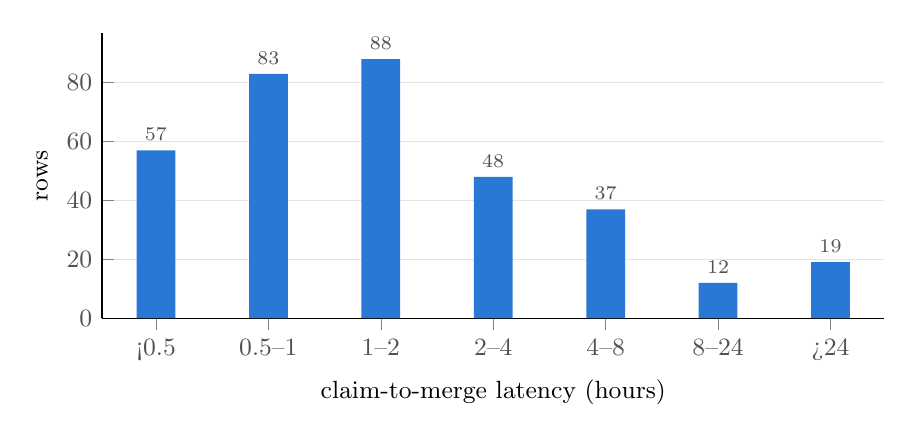
\begin{tikzpicture}
\begin{axis}[attbar,
  symbolic x coords={<0.5,0.5--1,1--2,2--4,4--8,8--24,>24},
  xtick=data, ylabel={rows}, xlabel={claim-to-merge latency (hours)}]
\addplot[fill=series, draw=none] coordinates {(<0.5,57) (0.5--1,83) (1--2,88) (2--4,48) (4--8,37) (8--24,12) (>24,19)};
\end{axis}
\end{tikzpicture}
\caption{Distribution of claim-to-merge latency for the 344 rows that were both claimed and merged.}
\label{fig:latency}
\end{figure}

\paragraph{Throughput.} Merged rows per day rose from 6--16 before the
supervisor (introduced on 2026-10-04) to a peak of 147 on 2026-10-05, the day
the leads began merging in trains (Figure~\ref{fig:throughput}). Of the 373
merged rows, 33 landed before the supervisor and 340 after it.

\begin{figure}[h]
\centering
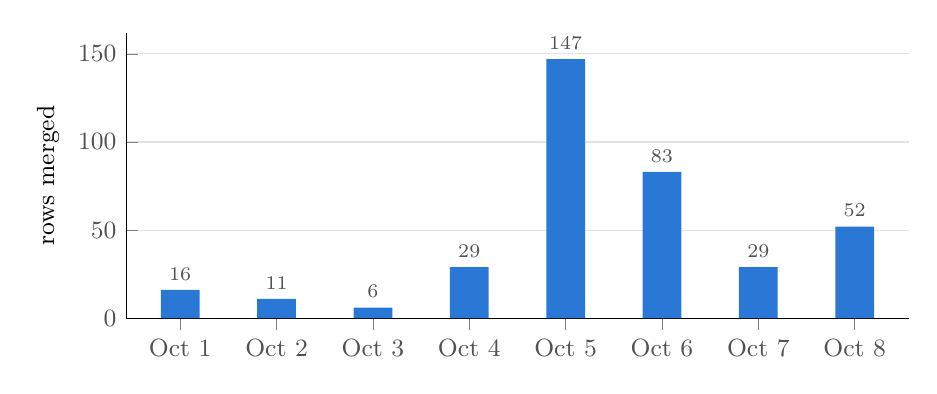
\begin{tikzpicture}
\begin{axis}[attbar,
  symbolic x coords={Oct 1,Oct 2,Oct 3,Oct 4,Oct 5,Oct 6,Oct 7,Oct 8},
  xtick=data, ylabel={rows merged}]
\addplot[fill=series, draw=none] coordinates {(Oct 1,16) (Oct 2,11) (Oct 3,6) (Oct 4,29) (Oct 5,147) (Oct 6,83) (Oct 7,29) (Oct 8,52)};
\end{axis}
\end{tikzpicture}
\caption{Backlog rows recorded as merged per day. The supervisor was introduced on Oct 4; merge trains on Oct 5. Oct 8 is a partial day.}
\label{fig:throughput}
\end{figure}

\paragraph{Before and after the supervisor.} For rows claimed before
2026-10-04, median claim-to-merge latency was 10.7\,h ($n{=}30$); for rows
claimed after it, 1.2\,h ($n{=}314$). Several things changed in the same days:
more agents, a second and third lead, staged CI that tests only what a PR
reaches, the quick test, and trains. We therefore read this as the
\emph{system} getting faster, not as an effect of the supervisor alone.

\paragraph{Who does the work.} By signed commits, leads authored 1{,}110,
supervised coders 726, the IDE-hosted coder 445, the PM agents 276 and cloud
sessions 169. The remaining 654 are the owner's, GitHub's merge commits, or
unsigned. Leads write the most commits because every review decision, row
state change and \emph{Merged} entry is a commit. The protocol records
decisions as data rather than as chat.

\section{What went wrong: the lessons}\label{sec:lessons}
The 83 lessons are the most transferable output of the deployment. Each is
dated and names the incident that taught it. Grouped by cause:

\begin{itemize}[leftmargin=*,itemsep=2pt]
\item \textbf{Shared state.} One process switching branches in a shared
  checkout put another agent's commits on the wrong branch, which led to
  per-agent worktrees. Unsigned commits led a lead to misread other sessions'
  merges as its own, which led to signed worktrees. Two leads reviewed the same
  PR, which led to label leases.
\item \textbf{CI semantics.} A draft's all-\texttt{SKIPPED} rollup read as
  ``pass''. A cancelled run on the same head read as ``fail''. A re-triggered
  run kept the old run's cancelled jobs. A PR run kept the workflow file of its
  old merge commit. A CI job that never installed a toolchain skipped every
  test that needed it and went green. Each became a guard in the merge script
  or a rule in the lead's skill.
\item \textbf{Resources.} Three coders' test suites, an orphaned application
  server and a supervisor test running together froze the 14\,GB machine. That
  led to ``the memory is the PM's'', capped quick tests, named memory scopes,
  and a self-hosted runner that leaves the queue while a live run is up.
\item \textbf{The evaluation gap.} Fixes that passed their unit tests did
  nothing on the real path (a function only the UI called), tuned themselves to
  the one reference input, or were scored as fixed by the product's own metric
  while failing on direct inspection. That led to ``check the path, not the
  function'', ``a fix's own score is not an output test'', and owner notes that
  close only when a live run shows them fixed.
\end{itemize}

\section{Limitations and threats to validity}\label{sec:limits}
This is a \emph{field study of one deployment}, not a controlled experiment.
(1) There is a single project, a single owner and nine days. (2) There is no
control arm: we do not compare against one agent, a human team, or ATT without
any one component. (3) The owner intervened throughout, setting priorities,
freezing the backlog and resizing the team. (4) Latency is measured from commit
timestamps; a row may have been worked on before its claim commit, and rows
merged outside the guarded path lack a \emph{Merged} commit. (5) Merged means
CI-green and lead-approved. It does not mean correct: rows wait in
\emph{Merged} until a live run confirms them, and we do not report the
confirmation rate here. (6) Commit counts are inflated by design, because every
decision is a commit. They measure activity, not productivity.

\section{Toward a controlled benchmark}\label{sec:future}
We propose evaluating ATT, and team architectures generally, on
\emph{backlog-level} rather than issue-level tasks. Start each run from a
frozen repository snapshot with a seeded backlog of $N$ rows of mixed levels,
some of which conflict in the files they touch, and a fixed machine and CI
budget. Run ATT, a single agent working the same backlog sequentially, and ATT
with one component removed (supervisor, leases, guarded merge, lessons).
Measure rows merged per wall-clock hour, regressions introduced on the
integration branch (by a held-out test suite), claim collisions, CI minutes per
merged row, and tokens per merged row. SWE-bench-style hidden tests can serve
as the held-out suite for each row.

\section{Conclusion}
A team of coding agents can run on one developer's machine and keep up with a
fast-moving product, provided the coordination is boringly explicit: one
backlog with one writer per part, claims as commits, leases as labels, merges
guarded on the reviewed head, short sessions with state on disk, and written
lessons. In one deployment this sustained a median of 1.3\,h from claim to
merge across 344 tasks. ATT packages that setup as a template, with every
project-specific value in one configuration file.

\paragraph{Availability.} \url{https://github.com/Alloooshe/ATT}

\paragraph{Acknowledgements.} The agents described here, and parts of this
manuscript's drafting, used Claude models through Claude Code. All numbers were
computed from the repository's git history with the script
\texttt{paper/analyze\_git\_history.py} in the ATT repository.

\bibliographystyle{plainnat}
\bibliography{refs}
\end{document}
